\subsection{Echo Hiding}

Jednym z najczęstszych podejść w dziedzinie steganografii audio jest metoda zwana \textit{Echo Hiding}, \textit{EH}. Metoda ta wykorzystuje właściwości dźwięku, dzięki którym dodatkowe echo można wprowadzić w sposób niesłyszalny dla ludzkiego ucha, jednocześnie kodując w nim wiadomość \cite{Gruhl1996EchoH}.

Podstawowa idea EH polega więc na dodaniu niewielkiego, kontrolowanego opóźnienia do oryginalnego sygnału audio. W celu zakodowania wiadomości, sygnał audio $x(n)$ poddawany jest operacji splotu z funkcją impulsową $h(n)$, która definiuje właściwości echa. Matematycznie proces ten można zapisać jako:
\begin{equation}
	y(n) = h(n) * x(n),
\end{equation}
gdzie operator $*$ oznacza splot, a $h(n)$ jest funkcją kernela zdefiniowaną jako:
\begin{equation}
	h(n) = \delta(n) + a \delta(n-d).
\end{equation}

W powyższym równaniu $\delta(n)$ oznacza funkcję delta Diraca, $a$ jest współczynnikiem tłumienia echa ($0 < a < 1$), a $d$ to opóźnienie echa wyrażone w próbkach.

Wartości $d$ oraz $a$ są zwykle dobierane w taki sposób, aby echo pozostało niesłyszalne, jednocześnie zapewniając wystarczające właściwości by umożliwić dekodowanie ukrytej wiadomości.

Przed kodowaniem, wejściowy sygnał audio dzieli się na segmenty o stałej długości $N$, w taki sposób, by każdy zawierał echo reprezentujące jeden bit wiadomości. Zamienia się więc ją na reprezentację binarną, a następnie koduje poprzez użycie dwóch różnych opóźnień: $d_0$, dla bitu "0", oraz $d_1$, dla bitu o wartości "1".

Zatem, osadzane dane są definiowane za pomocą czterech głównych parametrów echa (\ref{fig:echo-hiding}):
\begin{enumerate}
	\item amplituda echa ($A$),
	\item współczynnik zanikania ($\alpha$),
	\item opóźnienie dla bitu "1" (\textit{offset}),
	\item opóźnienie dla bitu "0" (\textit{offset + delta}).
\end{enumerate}

\begin{figure}[ht!]
	\centering
	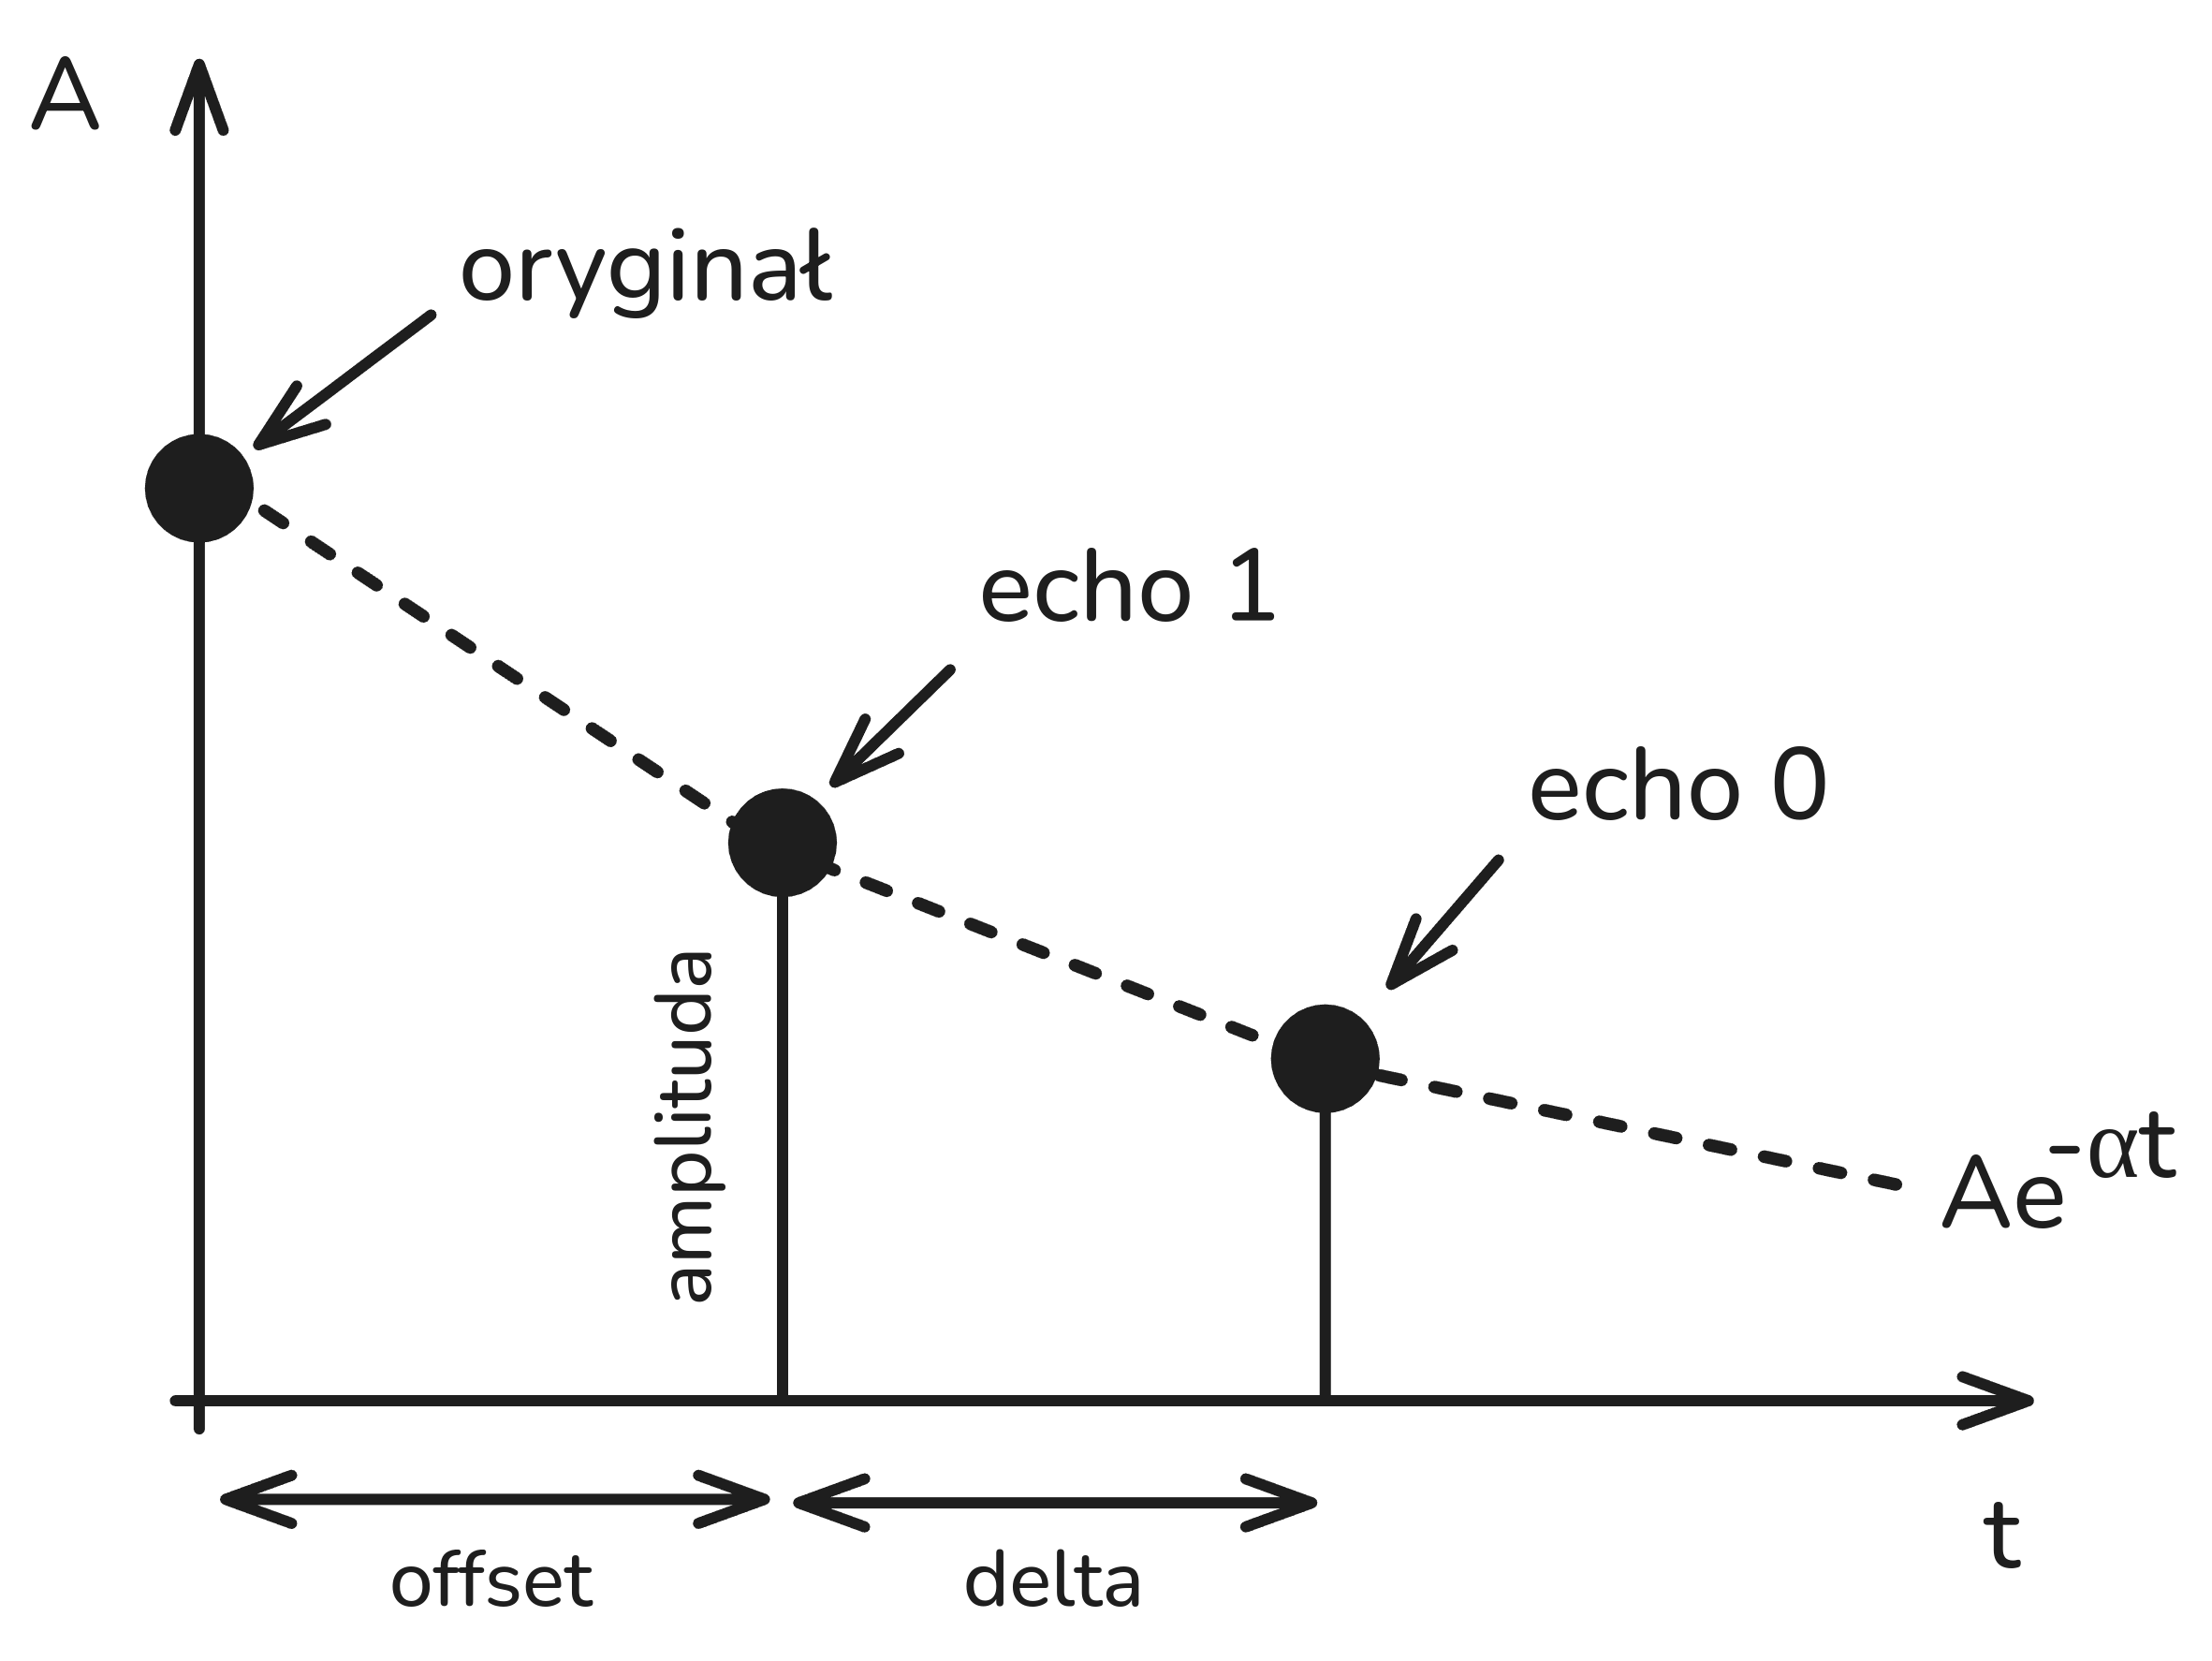
\includegraphics[width=0.8\textwidth]{img/echo-hiding.png}
	\caption{\label{fig:echo-hiding} Parametry EH}
\end{figure}
\pagebreak


\subsection{Dekodowanie}

\subsubsection{Analiza cepstralna i cepstrum mocy}

Najczęstszą procedurą wykorzystywaną do wykrywania echa jest analiza cepstralna.
Obliczenie tzw. cepstrum $C_y(n)$ pozwala zidentyfikować opóźnienia dodanego echa, ponieważ zawiera wyraźne szczyty w odpowiadających im pozycjach.

Cepstrum $C_y(n)$ definiowane jest jako odwrotna transformata Fouriera logarytmu widma amplitudowego sygnału:
\begin{equation}
	C_y(n) = \mathcal{F}^{-1} \big(\ln |\mathcal{F}(y(n))|\big),
\end{equation}
gdzie $\mathcal{F}$ oznacza transformatę Fouriera, $y(n)$ to sygnał z ukrytym echem, a $\mathcal{F}^{-1}$ oznacza odwrotną transformatę Fouriera.

Można również zdefiniować tzw. cepstrum mocy (ang. \textit{power cepstrum}), które daje lepsze wyniki niż samo cepstrum \cite{auto_power_cepstrum}. Oblicza się je jako odwrotną transformatę Fouriera logarytmu mocy widma sygnału:
\begin{equation}
	P_{\text{y}}(n) = \left| \mathcal{F}^{-1} \big( \ln |\mathcal{F}(y(n))|^2 \big) \right|^2,
\end{equation}

% TODO: plots: signal vs. spectrum vs. cepstrum vs. power cepsturm

\subsubsection{Estymacja parametrów}

Dokonując steganalizy jako potencjalny atakujący, nie mamy pojęcia o użytych parametrach do kodowania echem. Natomiast, możliwa jest ich estymacja poprzez wykorzystanie analizy cepstrum mocy z przesuwanym oknem (ang. \textit{sliding window}) \cite{echo_swc}.

W tej metodzie sygnał analizowany jest sekcja po sekcji za pomocą okna o określonym rozmiarze $\tau$, które przesuwa się po sygnale z krokiem $k$. Dla każdej sekcji obliczane jest cepstrum mocy, a następnie lokalizowane są szczyty odpowiadające potencjalnym opóźnieniom $d_0$ i $d_1$. Po przesunięciu okna przez cały sygnał tworzy się histogram lokalizacji szczytów w celu identyfikacji najbardziej prawdopodobnych wartości opóźnień.

% TODO: sliding window diagram

% TODO: code snippet for delay estimation
% TODO: peak location histogram

Kolejnym krokiem jest oszacowanie długości segmentów $N$, z jakimi zakodowana jest wiadomość. Odbywa się to poprzez analizę zmian amplitudy cepstrum mocy w miejscach $d_0$ i $d_1$. Kiedy okno przesuwa się przez granice sąsiednich segmentów, amplitudy w tych miejscach zmieniają się w charakterystyczny sposób. Punkty przecięcia amplitud w lokalizacjach $d_0$ i $d_1$ pozwalają oszacować odległość między granicami segmentów, co prowadzi do wstępnego oszacowania długości segmentu. Następnie długość segmentu może być doprecyzowana za pomocą tzw. \textit{grid search}, w którym optymalizuje się sumę amplitud cepstrum mocy w lokalizacjach $d_0$ i $d_1$.

% TODO: Wykres zmian amplitudy cepstrum mocy w lokalizacjach $d_0$ i $d_1$, przedstawiający punkty przecięcia i granice segmentów.

\subsection{Podsumowanie}

W ramach projektu zaimplementowano algorytmy pozwalające na detekcję opóźnień $d_0$ i $d_1$, oraz oszacowanie długości segmentów $N$. Kluczowe równania, takie jak obliczanie cepstrum mocy oraz proces analizy z przesuwanym oknem, zostały zaimplementowane w środowisku Python. Metody te zostały następnie przetestowane na różnych sygnałach audio.

% W kolejnych sekcjach dokumentacji omówiono szczegóły implementacji, wyniki testów oraz wnioski dotyczące skuteczności proponowanego podejścia.

\subsection{Analiza wyników}
